% vortrag.tex                   09 Oct 95
%------------------------------------------------------------

%
% Vortrag zur Studienarbeit -- makeindex4
%
% [LaTeX2e]



\documentclass[headrule,footrule,dvips,17pt]{foils}

\usepackage{german}
\usepackage{epsfig}
\usepackage{ifthen}

\newcommand{\ReportMode}{0}
\usepackage{stdwrk}
\usepackage{xindy}
\usepackage{bslash}


\newcommand{\IXLOGO}{\mbox{\normalfont%%
    \textbf{\huge\textsf{x\shortstack{{\normalsize$\circ$}\\\i}ndy}}}}
\newcommand{\ixlogo}{\mbox{\normalfont%%
    \textbf{\textsf{x\kern-2pt\shortstack{%%
          $\scriptscriptstyle\circ$\\[-2pt]\i}%%
        \kern-2pt ndy}}}}

\MyLogo{\ixlogo\ --- Institut f"ur Theoretische Informatik}

\parindent 0mm
\raggedright

\begin{document}

\title{\IXLOGO\\[2ex]
  {\rmfamily\textsl{Flexible Indexing System}}\\[2cm]%%
}
\author{%%
  {\small Studienarbeit}\\[1ex]
  Roger Kehr}
\date{\small 16.\ Oktober 1995}

\maketitle

\foilhead{Motivation}

\begin{center}
  \emph{Suchet so werdet ihr finden\ldots}
\end{center}

\vspace{3ex}

Grenzen von herk"ommlichen Indexierungssystemen

\begin{itemize}

\item Multinationale Indexe\\Definition und Sortierung von Alphabeten
\item Indexe mit Symbolen\\Sortierung
\item Referenzen auf strukturierte \emph{Lokationen} --- \\ bisher nur
  Seitennummern \\ aber: (\emph{Kapitel-3}, \emph{Anhang-C},
  \emph{7--3})
\item Erweiterte W"unsche bei der
  Ausgabeformatierung\\verschiedenartige Ausgabeformen gew"unscht
\end{itemize}

\foilhead{"Uberblick}

\begin{itemize}
\item Aufgaben eines Indexierungssystems
\item Datenflu�
\item Analyse
\item Modellentwurf
\item Implementierung
\item Zusammenfassung und Ausblick
\end{itemize}

\vspace{3ex}

\emph{Was macht eine Indexierungssystem~?}

$\Rightarrow$\quad Automatische Generierung eines Indexes aus Rohdaten

\begin{itemize}
\item Einlesen von Indexierungsinformationen
\item Sortieren und mischen von Stichw"ortern
\item Zusammenfassen von Lokationsreferenzen zu Bereichen
\item Ausgabeformatierung --- Markup
\end{itemize}


\foilhead{Datenflu� in einem Indexierungssystem}

{\hfill\mbox{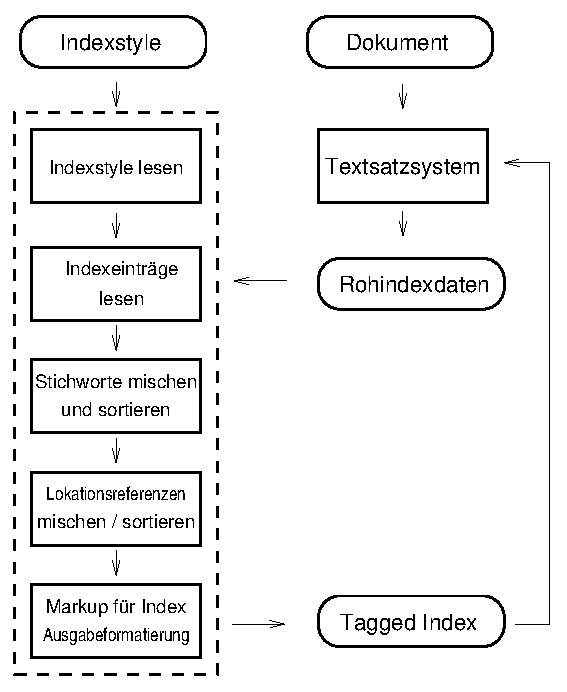
\epsfig{file=datenfluss.eps,width=14cm}}\hfill}

\foilhead{Beispiel-Index}

\begin{center}
  \begin{minipage}{15cm}%
      \begin{mkindex}
        \idx B�ume
        \subidx AVL, \textbf{23}, 22--25, 38
        \subidx nat�rliche, {\bfseries 20}, 18--21
        \idx Fibonacci Queues, \emph{siehe} Priority Queues
        \idx Suche
        \subidx bin�re, {\bfseries 5}, 4--7, 11
        \subidx sequentielle, {\bfseries 7}, 6--8, 10
        \subsubidx geordnete, 6, \emph{siehe auch} ungeordnete Suche
        \subsubidx ungeordnete, 7
        \idx Priority Queues
        \subidx Fibonacci, {\bfseries 35--36}, 41\emph{f.}%
      \end{mkindex}%
    \end{minipage}%
\end{center}

\textbf{Grundelemente:}

\begin{itemize}
\item Stichw"orter
\item Lokationsreferenzen
\end{itemize}

$\Rightarrow\quad$  Stichw"orter haben eine \emph{hierarchische} Struktur

\begin{description}
\item[Notation]\mbox{}\\
  {\tt (}
  \Arg{Ebene$_{1}$} {\tt :} \Arg{Ebene$_{2}$} {\tt :}
  \ldots{} {\tt :} \Arg{Ebene$_{n}$}
  {\tt )}

  \bigskip

  $\Rightarrow\quad$\Hierzwei{B"aume}{nat"urliche}

\end{description}



\foilhead{Stichwortverarbeitung}
\begin{description}
\item[Aufgaben] \mbox{}\\
  \begin{itemize}
  \item Sortieren
  \item Mischen
  \end{itemize}

\item[Probleme]\mbox{}\\
  \begin{itemize}
  \item Uneinheitliche orthographische Regeln
  \item Verschiedenartige Alphabete
  \item Gleichheitsbegriff \\ Wann sind zwei Stichw"orter \emph{gleich}?
  \end{itemize}

\item[L"osungen]\mbox{}\\
  \begin{itemize}
  \item Normalisierung mittels
    \begin{itemize}
    \item \emph{sort-mapping}
    \item \emph{merge-mapping}
    \end{itemize}
    Mappings werden durch Regul"are Ausdr"ucke und Substitutionsmuster
    definiert

    Beispiel: \texttt{"a} $\rightarrow$ \texttt{ae}
  \item Konfigurierung durch den Benutzer
  \item Implementiert im \textit{International MakeIndex}
  \end{itemize}
\end{description}


\foilhead{Lokationsreferenzen}

\emph{Was gibt es f"ur Arten von Lokationsreferenzen~?}

\begin{itemize}
\item \emph{Seitennummern}:

  11, 12, 13, \ldots

  iii, iv, v, \ldots

\item \emph{Gliederungsnummern}:

  1.1, 1.2, 1.2.1, 1.2.2, \ldots

  1a, 1b, \ldots

\item \emph{Kapitelseiten}: 7--3, 7--4, \ldots

\item \emph{Gesetzb"ucher}: \textbf{1} \S436

\item \emph{Abschnitte}: Anhang-A, Kapitel-3, \ldots
\end{itemize}

\begin{description}

\item[Ergebnis]\mbox{}\\
  \begin{itemize}
  \item Lokationsreferenzen besitzen eine \emph{hierarchische} Struktur
  \item \emph{Trennzeichen} trennen \emph{Strukturebenen} voneinander
    ab
  \end{itemize}
  \bigskip

\item[Notation]\mbox{}\\
  \Strukdrei{\textsl{Ebene$_{1}$}}{\textsl{Trenner$_{1}$}}%
  {\ldots}     {\textsl{Trenner$_{n-1}$}}%
  {\textsl{Ebene$_{n}$}}

\end{description}


\foilhead{Strukturebenen}

Strukturebenen bilden sich aus den folgenden Kategorien:

\begin{itemize}
\item \emph{Aufz"ahlungen}\\ wie z.B.\ alle Arten von Nummern
\item \emph{Alphabete}\\ wie z.B.\ Buchstaben, Begriffe, etc.
\end{itemize}

Die Kategorien von Strukturebenen werden mit \emph{Komponententypen}
bezeichnet.

\begin{description}
\item[Beispiele]\mbox{}\\
  \begin{itemize}
  \item Arabische Zahlen (\texttt{num}), kleine/gro"se r"omische
    Zahlen (\texttt{roman}/\texttt{ROMAN}), etc.
  \item kleines/gro"ses lateinisches Alphabet
  (\texttt{alpha}/\texttt{ALPHA}), Begriffe
  (\quasi{Anhang},\quasi{Kapitel}), etc.
  \end{itemize}
\end{description}


\foilhead{Lokationsklassen}

Durch \emph{Komposition} von Komponententypen k"onnen
\emph{Lokationsklassen} gebildet werden.

\begin{description}
\item[Beispiel]\mbox{}\\
  \begin{itemize}
  \item Seitennummern: \Strukeins{\texttt{num}}
  \item Gliederungsnummern:
    \Strukdrei{\texttt{num}}{.}{\texttt{num}}{.}{\texttt{num}}
  \item Gemischt: \Strukzwei{\texttt{roman}}{}{\texttt{alpha}}
  \end{itemize}
\item[Problem] \mbox{}\\ \emph{Vertr"aglichkeit} der Zeichenmengen\\%
  \texttt{roman} ist echte Untermenge von \texttt{alpha}
\item[L"osung] \mbox{}\\
  \begin{enumerate}
  \item Trennzeichen verwenden
  \item Dummy-Pr"afixe einf"uhren
  \end{enumerate}
\end{description}

\foilhead{Lokationsklassentypen und deren Zuordnungsstrategien}

\begin{itemize}
\item \emph{Standardklassen}
  \begin{itemize}
  \item Die Struktur der Klasse ist fest vorgegeben
  \item Beispiel: \Strukzwei{\texttt{ALPHA}}{--}{\texttt{num}}
  \item Eine Zeichenkette mu"s komplett auf die Klassenstruktur passen
  \end{itemize}
\item \emph{Varklassen}
  \begin{itemize}
  \item Bilden einen Verband von einfachen Klassen
  \item Beispiel: Gliederungsnummern der Form\\%%
    \quad \Strukdrei{\texttt{num}}{.}{\texttt{num}}{.}{\texttt{num}}\\%%
    enth"alt insgesamt drei einfache Klassen.
  \item Zuordnungsstrategie: \emph{Pr"afixzuordnung}
  \item Notation im folgenden:\\%%
    \quad
    \Metaclass{\Strukdrei{\texttt{num}}{.}{\texttt{num}}{.}{\texttt{num}}}
  \end{itemize}
\end{itemize}


\foilhead{Kategorieattribute}

\emph{Lokationskategorien}

Verweise auf \emph{Definitionen}, \emph{Verwendungen},
\emph{Beispiele} etc.

\begin{center}
  Suche, bin"are, 10-17, \textbf{14}, \emph{12}
\end{center}


$\Rightarrow\quad$ Zuweisung eines \emph{Kategorieattributs}

Auswirkungen auf:
\begin{itemize}
\item Sortierreihenfolge
\item Bereichsbildung
\item Ausgabeformatierung
\end{itemize}



\foilhead{Sortieren von Lokationsreferenzen\\---\\Totale Ordnung}

\emph{Wie ist die \emph{Ordnung} ?}

Die Ordnung wird ben"otigt, um die Lokationsreferenzen zu sortieren.

Ordnungskriterien:

\begin{itemize}
\item Lokationsklassen\\
  \Strukeins{\texttt{num}} $<$ \Strukzwei{\texttt{ALPHA}}{--}{\texttt{num}}
\item Implizite Ordnung innerhalb einer Lokationsklasse\\
  \Strukeins{11} $<$ \Strukeins{12}\\
  \Metaclass{\Strukzwei{1}{.}{2}} $<$ \Metaclass{\Strukdrei{1}{.}{2}{.}{1}}
\end{itemize}

$\Rightarrow\quad$ Die Totale Ordnung l"a"st sich auf die Ordnung der
Komponententypen zur"uckf"uhren


\foilhead{Mischen von Lokationsreferenzen\\---\\Direkter Nachfolger}

\emph{Was ist ein \emph{Nachfolger}~?}

Der Nachfolger wird ben"otigt, um Bereiche zu bilden.

\newcommand{\Succ}[1]{{\textit{succ}\mbox{$($}\mbox{#1}\mbox{$)$}}}

\begin{description}
\item[Problem]\mbox{}\\
  Welche Lokationsreferenz ist die \emph{nachfolgende} ?

  \Succ{\quasi{11}} = \quasi{12}, \Succ{\quasi{A--1}} = \quasi{A--2}
  etc.

  aber:

  \Succ{\quasi{1.2}} = \quasi{1.2} oder \quasi{1.2.1}, \quasi{1.2.0}
  ???

  Fehlendes Wissen "uber die Dokumentstruktur !

\item[L"osung]\mbox{}\\
  Dieses \emph{Dokumentwissen} mu"s dem System explizit zugef"uhrt
  werden !

  Dies kann z.B.\ aus einer Menge von Nachfolger-\emph{Deklarationen}
  bestehen

  $\Rightarrow\quad$ \Succ{\quasi{1.2}} $\stackrel{\normalfont
    def}{\equiv}$ \quasi{1.2.1}
\end{description}


\rotatefoilhead{Sortieren und Mischen mit Attributen}
\begin{center}
  \small
  \begin{tabular}{|c|c|c|c|c|c|c|l|}
    \hline
    \medrule\textsl{Nr.} & \textsl{Typ} &
    \multicolumn{4}{|c|}{\textsl{Bereiche}} &
    \textsl{Lokationsreferenzen}\\ \hline
    & \textsf{Sep} & ohne & \multicolumn{3}{|c|}{einfach} &\\ \cline{5-6}
    & oder & & & \multicolumn{2}{|c|}{\small zugeordnet} &
    11 13 14 15 17 25\ \textbf{12 15 25}\\ \cline{6-6}
    & \textsf{Mix} & & & &{\footnotesize unterdr�ckt} &\\
    \hline\hline
    1 & \textsf{Sep} &$\circ$& & & & 11 13 14 (15) 17 (25)\ \textbf{12 15 25} \\
    2 & \textsf{Sep} & &$\circ$& & & 11 13--15 17 (25)\ \textbf{12 15 25} \\
    3 & \textsf{Sep} & & &$\circ$& & 11--15 17 (25)\ \textbf{12 15 25} \\
    4 & \textsf{Sep} & & & &$\circ$& 11--15 17 (25)\ \textbf{25} \\
    \hline
    5 & \textsf{Mix} &$\circ$& & & & 11 \textbf{12} 13 14 \textbf{15} 17
    \textbf{25}\\
    6 & \textsf{Mix} & &$\circ$& & & 11 \textbf{12} 13--15 \textbf{15} 17
    \textbf{25}\\
    7 & \textsf{Mix} & & &$\circ$& & 11--15 \textbf{12 15} 17 \textbf{25}\\
    8 & \textsf{Mix} & & & &$\circ$& 11--15 17 \textbf{25} \\
    \hline%
  \end{tabular}%
\end{center}

\bigskip

Um die gew"unschten Ausgabevarianten zu realisieren, gibt es einen
Satz von \emph{Regeln} mit fest definierter Semantik.



\foilhead{Ausgabeformatierung}

\textbf{Ziele:}
\begin{itemize}
\item Stichw"orter und Unterstichw"orter werden geeignet ausgegeben
\item Lokationsreferenzen werden klassenweise ausgegeben

  \emph{Wichtig: Lokationsreferenzen bilden keine Einheit !}

  Beispiel Gesetzb"ucher: \textbf{1} \S436

\item Textsatzsysteme benutzen \emph{Umgebungen}

  \emph{siehe} \TeX{}: \underline{\texttt{\bslash
      textit\{}} \texttt{siehe} \underline{\texttt{\}}}

\item \emph{Wiederholungssymbole}:

  \begin{tabbing}
    \hspace{1cm}\=S\=uche\=, bin�re \hspace{3em} \=\ldots\\
    \>\>$\widetilde{\ \ \ }$\>, sequentielle \>\ldots
  \end{tabbing}

\end{itemize}


\rotatefoilhead{Ausgabeformatierung}

\hfill
{\small
  \begin{tabular}{|c|c|c|c|c|c|c|c|c|}
    \hline%
    \multicolumn{9}{|c|}{\textbf{Ausgabematrix}\medrule}\\
    \hline\hline
    \multicolumn{9}{|c|}{\smallrule Ausgabeform:\, 1.1.1, 1.1.2,
      1.2.1--1.2.3, \ldots{} 2.1.1 \ldots{} $x.y.z$}\\
    \hline%
    \textit{Typ} & \textsf{pre-} &
    \textsf{pre-} & \textsf{layer} & \textsf{rep.-} & \textsf{post-} &
    \multicolumn{2}{|c|}{\textsf{optional-}} & \textsf{post-} \\[-2pt]
    & \textsf{node} & \textsf{layer} & & \textsf{symbol} & \textsf{layer} &
    \textsf{post-layer} & \textsf{range} & \textsf{node} \\
    \hline%
    \textsf{P}  & &                    & \textit{num} & & &
    \quasi{\textbf{,}$\sqcup$} & &\\
    \textsf{P} & & \quasi{\textbf{.}} & \textit{num} & & & & &\\
    \textsf{P} & & \quasi{\textbf{.}} & \textit{num} & & & &
    \quasi{\textbf{--}} &\\
    \hline%
    \hline%
    \multicolumn{9}{|c|}{\smallrule Ausgabeform:\, \textbf{1} 1.1, 1.2,
      2.1--2.3, \ldots{}; \textbf{2} $x.y$, \ldots{}}\\
    \hline%
    \textit{Typ} & \textsf{pre-} &
    \textsf{pre-} & \textsf{layer} & \textsf{rep.-} & \textsf{post-} &
    \multicolumn{2}{|c|}{\textsf{optional-}} & \textsf{post-} \\[-2pt]
    & \textsf{node} & \textsf{layer} & & \textsf{symbol} & \textsf{layer} &
    \textsf{post-layer} & \textsf{range} & \textsf{node} \\
    \hline%
    \textsf{A} & & {\small\slshape bold-on} & \textit{num} & &
    {\small\slshape bold-off} & \quasi{\textbf{;}$\sqcup$} & &\\
    \textsf{P} & \quasi{$\sqcup$} & & \textit{num} & & &
    \quasi{\textbf{,}$\sqcup$} & &\\
    \textsf{P} & & \quasi{\textbf{.}} & \textit{num} & & & &
    \quasi{\textbf{--}} &\\
    \hline
  \end{tabular}
}%
\hfill

\foilhead{Implementierung}


\begin{description}
\item[Ziele]\mbox{}\\
  \begin{itemize}
  \item schnelle Umsetzung --- Prototyping
  \item Verwendung in der \TeX-Umgebung
  \item hohe Portabilit"at
  \item hohe Konfigurierbarkeit
  \end{itemize}

  \vspace{3ex}

\item[Implementierung]\mbox{}\\
  \begin{itemize}
  \item \textsc{Common Lisp} mit CLOS f"ur Kernapplikation
    \begin{itemize}
    \item \texttt{clisp}-Interpreter (frei verf"ugbar)
    \item Portierung auf DOS etc.\ ohne Probleme
    \item viele Datenstrukturen sind Listen und Stacks
    \end{itemize}
  \item \texttt{perl}-Frontend als Parser
  \item Indexstyle als \textsc{Lisp}-Ausdr"ucke
  \item Literate-Programming-System \texttt{noweb} zur Dokumentation
  \end{itemize}

\end{description}


\foilhead{Zusammenfassung}
\begin{description}
\item[Zusammenfassung] \mbox{}\\
  \begin{itemize}
  \item Neuanalyse der Struktur von Indexen
  \item Schwerpunkt: Lokationsreferenzen
  \item hohe Konfigurierbarkeit
  \item kurze Implementierungszeit
  \item Probleme:
    \begin{itemize}
    \item Dokumentwissen
    \item Ausgabeformatierung
    \item Kategorieattribute
    \end{itemize}
  \end{itemize}

  \vspace{3ex}

\item[Weiterf"uhrende Arbeiten]\mbox{}\\

  \begin{itemize}
  \item Dokumentwissen und -struktur
  \item \emph{K"onnen Indexe dadurch besser werden~?}
  \item textsatzabh"angige Ausgabe\\%%
    Wiederholungssymbole etc.
  \item Untersuchung der Kopplung von Textsatzsystem und
    Indexierungssystem
  \end{itemize}
\end{description}


\end{document}
